
\documentclass[usenames, dvipsnames, tikz]{standalone}

\usepackage{tikz}
\usetikzlibrary{calc}

\begin{document}
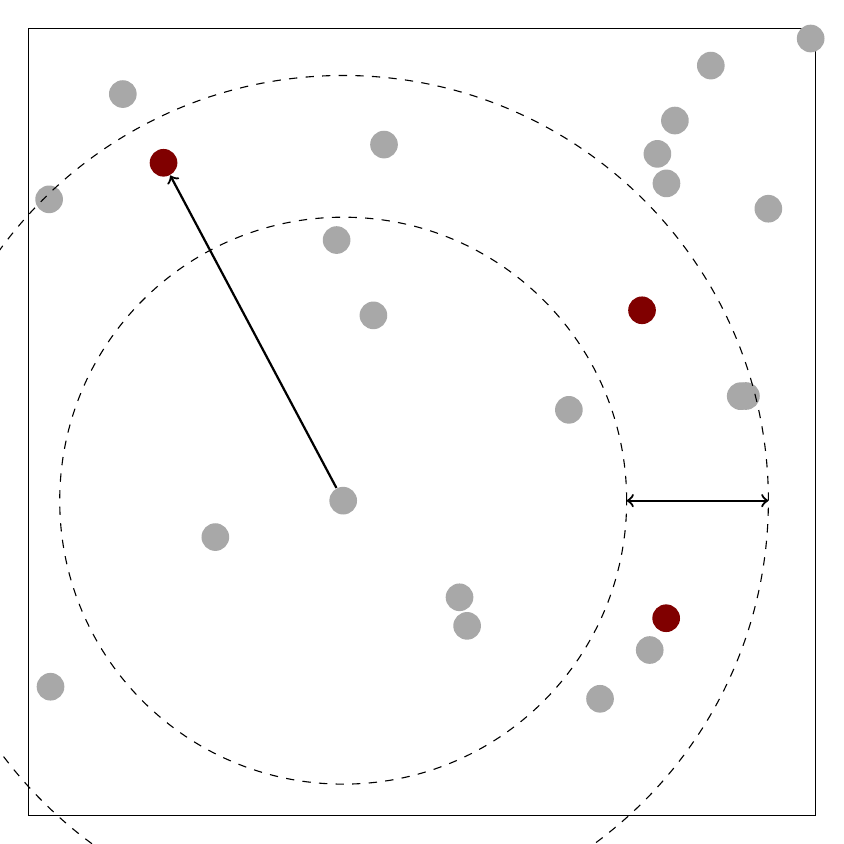
\begin{tikzpicture}[outmargin_node/.style={circle, inner sep=0,
    minimum size=10., fill=gray!68}, inmargin_node/.style={circle,
    inner sep=0, minimum size = 10., fill=Maroon}]

  \def \Edge {10.}
  \def \Distance {4.5}
  \def \Margin {0.9}

  \pgfmathsetseed{155}


  \draw[use as bounding box] (0,0) rectangle (\Edge,\Edge);

  \node[outmargin_node]
  (Origin) at (4,4) {};

   \foreach \i in {1,2,...,20}{
    \pgfmathsetmacro{\X}{rnd*\Edge}
    \pgfmathsetmacro{\Y}{rnd*\Edge)}

    \node[outmargin_node] at
    (\X,\Y) {};
    }


  % \node[draw, circle, inner sep=0, minimum size=10, fill=gray!25]
  % (t_1) at (7,4) {};

  \node[inmargin_node] (Target) at
  ($(Origin) +(32.5:\Distance)$) {};

  \node[inmargin_node] (t1) at
  ($(Origin) +(118:\Distance+\Margin*0.4)$) {};

  \node[inmargin_node] (t2) at
  ($(Origin) +(340:\Distance-\Margin*0.15)$) {};
 

  \draw[dashed] (Origin) circle (\Distance+\Margin);
  \draw[dashed] (Origin) circle (\Distance-\Margin);

  \draw[thick, ->] (Origin) -- (t1);

  \draw[thick, <->] ($(Origin)+(\Distance-\Margin,0)$) --
  ($(Origin)+(\Distance+\Margin,0)$);


\end{tikzpicture}
\end{document}
%%% Local Variables: 
%%% mode: latex
%%% TeX-master: t
%%% End: 
